\iffalse
\documentclass[journal,12pt,twocolumn]{IEEEtran}
\usepackage{setspace}
\usepackage{gensymb}
\singlespacing
\usepackage[cmex10]{amsmath}
\usepackage{amsthm}
\usepackage{mathrsfs}
\usepackage{txfonts}
\usepackage{stfloats}
\usepackage{bm}
\usepackage{cite}
\usepackage{cases}
\usepackage{subfig}
\usepackage{longtable}
\usepackage{multirow}
\usepackage{enumitem}
\usepackage{mathtools}
\usepackage{steinmetz}
\usepackage{tikz}
\usepackage{circuitikz}
\usepackage{verbatim}
\usepackage{tfrupee}
\usepackage[breaklinks=true]{hyperref}
\usepackage{tkz-euclide}
\usetikzlibrary{calc,math}
\usepackage{listings}
    \usepackage{color}                                            %%
    \usepackage{array}                                            %%
    \usepackage{longtable}                                        %%
    \usepackage{calc}                                             %%
    \usepackage{multirow}                                         %%
    \usepackage{hhline}                                           %%
    \usepackage{ifthen}                                           %%
  %optionally (for landscape tables embedded in another document): %%
    \usepackage{lscape}     
\usepackage{multicol}
\usepackage{chngcntr}
\DeclareMathOperator*{\Res}{Res}
\renewcommand\thesection{\arabic{section}}
\renewcommand\thesubsection{\thesection.\arabic{subsection}}
\renewcommand\thesubsubsection{\thesubsection.\arabic{subsubsection}}

\renewcommand\thesectiondis{\arabic{section}}
\renewcommand\thesubsectiondis{\thesectiondis.\arabic{subsection}}
\renewcommand\thesubsubsectiondis{\thesubsectiondis.\arabic{subsubsection}}

% correct bad hyphenation here
\hyphenation{op-tical net-works semi-conduc-tor}
\def\inputGnumericTable{}                                 %%

\lstset{
frame=single, 
breaklines=true,
columns=fullflexible
}

\begin{document}


\newtheorem{theorem}{Theorem}[section]
\newtheorem{problem}{Problem}
\newtheorem{proposition}{Proposition}[section]
\newtheorem{lemma}{Lemma}[section]
\newtheorem{corollary}[theorem]{Corollary}
\newtheorem{example}{Example}[section]
\newtheorem{definition}[problem]{Definition}
\newcommand{\BEQA}{\begin{eqnarray}}
\newcommand{\EEQA}{\end{eqnarray}}
\newcommand{\define}{\stackrel{\triangle}{=}}

\bibliographystyle{IEEEtran}
\providecommand{\mbf}{\mathbf}
\providecommand{\pr}[1]{\ensuremath{\Pr\left(#1\right)}}
\providecommand{\qfunc}[1]{\ensuremath{Q\left(#1\right)}}
\providecommand{\sbrak}[1]{\ensuremath{{}\left[#1\right]}}
\providecommand{\lsbrak}[1]{\ensuremath{{}\left[#1\right.}}
\providecommand{\rsbrak}[1]{\ensuremath{{}\left.#1\right]}}
\providecommand{\brak}[1]{\ensuremath{\left(#1\right)}}
\providecommand{\lbrak}[1]{\ensuremath{\left(#1\right.}}
\providecommand{\rbrak}[1]{\ensuremath{\left.#1\right)}}
\providecommand{\cbrak}[1]{\ensuremath{\left\{#1\right\}}}
\providecommand{\lcbrak}[1]{\ensuremath{\left\{#1\right.}}
\providecommand{\rcbrak}[1]{\ensuremath{\left.#1\right\}}}
\theoremstyle{remark}
\newtheorem{rem}{Remark}
\newcommand{\sgn}{\mathop{\mathrm{sgn}}}
\providecommand{\abs}[1]{\left\vert#1\right\vert}
\providecommand{\res}[1]{\Res\displaylimits_{#1}} 
\providecommand{\norm}[1]{\left\lVert#1\right\rVert}
\providecommand{\mtx}[1]{\mathbf{#1}}
\providecommand{\mean}[1]{E\left[ #1 \right]}
\providecommand{\fourier}{\overset{\mathcal{F}}{ \rightleftharpoons}}
\providecommand{\system}{\overset{\mathcal{H}}{ \longleftrightarrow}}
\newcommand{\solution}{\noindent \textbf{Solution: }}
\newcommand{\cosec}{\,\text{cosec}\,}
\providecommand{\dec}[2]{\ensuremath{\overset{#1}{\underset{#2}{\gtrless}}}}
\newcommand{\myvec}[1]{\ensuremath{\begin{pmatrix}#1\end{pmatrix}}}
\newcommand{\mydet}[1]{\ensuremath{\begin{vmatrix}#1\end{vmatrix}}}
\numberwithin{equation}{subsection}
\makeatletter
\@addtoreset{figure}{problem}
\makeatother

\let\StandardTheFigure\thefigure
\let\vec\mathbf
\renewcommand{\thefigure}{\theproblem}



\def\putbox#1#2#3{\makebox[0in][l]{\makebox[#1][l]{}\raisebox{\baselineskip}[0in][0in]{\raisebox{#2}[0in][0in]{#3}}}}
     \def\rightbox#1{\makebox[0in][r]{#1}}
     \def\centbox#1{\makebox[0in]{#1}}
     \def\topbox#1{\raisebox{-\baselineskip}[0in][0in]{#1}}
     \def\midbox#1{\raisebox{-0.5\baselineskip}[0in][0in]{#1}}

\vspace{3cm}


\title{Assignment 1}
\author{Jaswanth Chowdary Madala}





% make the title area
\maketitle

\newpage

%\tableofcontents

\bigskip

\renewcommand{\thefigure}{\theenumi}
\renewcommand{\thetable}{\theenumi}


\begin{enumerate}

\textbf{Solution:}
\fi
The input parameters are available in Table 
\ref{tab:chapters/9/10/5/10/1}.
\begin{table}[h]
\centering
%%%%%%%%%%%%%%%%%%%%%%%%%%%%%%%%%%%%%%%%%%%%%%%%%%%%%%%%%%%%%%%%%%%%%%
%%                                                                  %%
%%  This is a LaTeX2e table fragment exported from Gnumeric.        %%
%%                                                                  %%
%%%%%%%%%%%%%%%%%%%%%%%%%%%%%%%%%%%%%%%%%%%%%%%%%%%%%%%%%%%%%%%%%%%%%%
\begin{center}
\begin{tabular}{|c|c|c|}
\hline
\textbf{Parameter}	&\textbf{Description}& \textbf{Value}\\ \hline
$\vec{A}	$ & vertex of the triangle &	$\myvec{0\\4}$ 	\\ \hline
$\vec{B}	$ & vertex of the triangle &	$\myvec{0\\-4}$	\\ \hline
$\vec{C}$ &vertex of the triangle  &	$\myvec{6\\6}$\\ \hline
\end{tabular}
\end{center}
\caption{}
\label{tab:chapters/9/10/5/10/1}
\end{table}
The equation of circle taking $AB$ as diameter is given by,
\begin{align}
\norm{\vec{x}}^2 + 2\vec{u_1}^\top\vec{x} + f_1 &= 0 \\
\implies 
\norm{\vec{x}}^2 -16 &= 0
\label{eq:chapters/9/10/5/10/1}
\end{align}
where
\begin{align}
\vec{u_1} = -\brak{\frac{\vec{A}+\vec{B}}{2}}
&= \myvec{0\\0}\\
r_1 = \frac{\norm{\vec{A}-\vec{B}}}{2}
&= 4\\
f_1 = \norm{\vec{u_1}}^2 - r_1^2
&= -4
\end{align}
The equation of circle taking $AC$ as diameter is given by,
\begin{align}
\norm{\vec{x}}^2 + 2\vec{u_2}^\top\vec{x} + f_2 &= 0 \\
\implies \norm{\vec{x}}^2 -2\myvec{3&5}\vec{x}+24 &= 0
\label{eq:chapters/9/10/5/10/2}
\end{align}
where
\begin{align}
\vec{u_2} = -\brak{\frac{\vec{A}+\vec{C}}{2}}
&= -\myvec{3\\5}\\
r_2 = \frac{\norm{\vec{A}-\vec{C}}}{2}
&= \sqrt{10}\\
f_2 = \norm{\vec{u_2}}^2 - r_2^2
&= 24
\end{align}
Let the intersection of circles \eqref{eq:chapters/9/10/5/10/1} and \eqref{eq:chapters/9/10/5/10/2} be $\vec{P}$. The equation of the common chord of intersection of two circles, $AP$ is given by,
\begin{align}
2\vec{u_1}^\top\vec{x}-2\vec{u_2}^\top\vec{x}+f_1 - f_2 &= 0\\
\implies
2\myvec{3 & 5}\vec{x}-16-24&= 0\\
\myvec{3&5}\vec{x} &= 20
\label{eq:chapters/9/10/5/10/3}
\end{align}
\eqref{eq:chapters/9/10/5/10/3} can be written in parametric form as,
\begin{align}
	\vec{x} =  \vec{h}+ \mu \vec{m}, \text{ where }
\vec{h} = \myvec{0\\4}, \, \vec{m} = \myvec{-5\\3}
\end{align}
and $\mu$ 
is given by 
\begin{align}
\mu^2\vec{m}^{\top}\vec{V}\vec{m} + 2 \mu\vec{m}^{\top}\brak{\vec{V}\vec{h}+\vec{u}} + \text{g}\brak{\vec{h}} &=0
\label{eq:chapters/9/10/5/10/6}
\end{align}
with
\begin{align}
\text{g}\brak{\vec{h}} &= \vec{h}^{\top}\vec{V}\vec{h}+2\vec{u}^{\top}\vec{h}+f
\label{eq:chapters/9/10/5/10/5}
\end{align}
Substituting
\begin{align}
\vec{V} = \vec{I}, \, \vec{u} = \myvec{0\\0}, \, f = 16
\vec{h} = \myvec{0\\4}, \, \vec{m} = \myvec{-5\\3}
\end{align}
\begin{align}
34\mu^2 + 24 \mu = 0 \implies
\mu = 0, -\frac{12}{17}
\end{align}
where
$\mu = 0$ corresponds to point $\vec{A}$.
Thus, 
\begin{align}
\vec{P} = \myvec{0\\4} -\frac{12}{17} \myvec{-5\\3}
 = \myvec{\frac{60}{17}\\\\\frac{32}{17}}
\end{align}
The direction vector of $BC$ is given by,
\begin{align}
\vec{m} = \vec{C}-\vec{B}
= \myvec{3\\5}
\implies \vec{n} = \myvec{-5\\3}
\end{align}
yielding the equation 
\begin{align}
\vec{n}^\top\vec{x} &= \vec{n}^\top\vec{B}
\\
\implies \myvec{-5&3}\vec{x} &= \myvec{-5&3}\myvec{0\\-4}
= -12
\label{eq:chapters/9/10/5/10/7}
\end{align}
It is clear that $\vec{P}$ satisfies the equation of ${BC}$ in \eqref{eq:chapters/9/10/5/10/7}. Hence, the point of intersection of the circles drawn by taking two sides of a triangle as diameters lies on the third side.
See Fig. 
\ref{fig:chapters/9/10/5/10/1}.
\begin{figure}[ht]
\centering
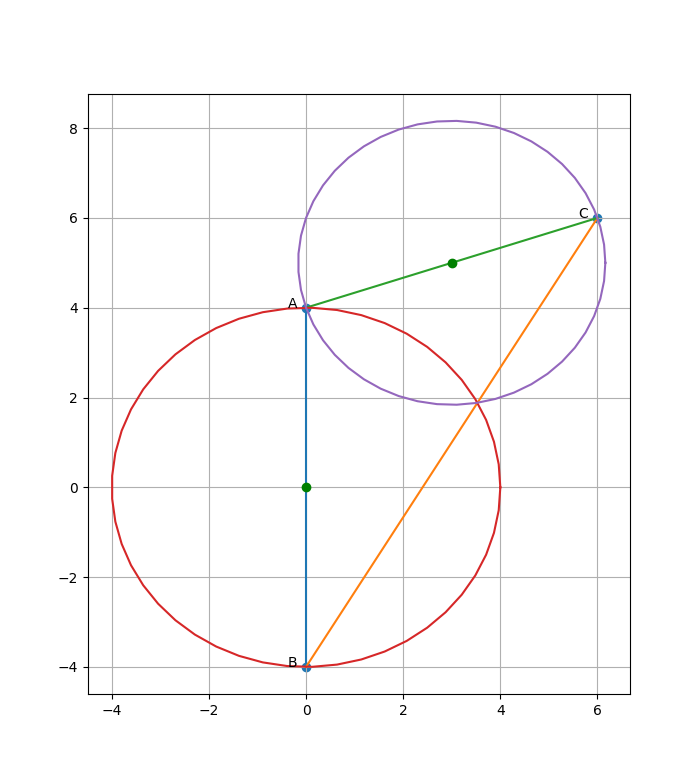
\includegraphics[width = \columnwidth]{chapters/9/10/5/10/figs/fig.png}
\caption{Graph}
\label{fig:chapters/9/10/5/10/1}
\end{figure}

